%! Author = Sujal Singh
%! Date = 11/3/23

% Preamble
\documentclass[12pt]{ipu-mechanics}
\title{Engineering Mechanics\\[10pt]Assignment--1}

% Packages
\usepackage{amsmath}
\usepackage{mathtools}
\usepackage{bm}
\usepackage[
    pdftitle={Engineering Mechanics Assignment 1},
    pdfsubject={Engineering Mechanics Assignment 1},
    pdfauthor={Sujal Singh},
    pdfdisplaydoctitle,
    hidelinks,
]{hyperref}
\usepackage{tikz}
\usepackage{wrapfig}
\usepackage{amssymb}
\usepackage{gensymb}
\usepackage[shortlabels]{enumitem}

\usetikzlibrary{angles,arrows.meta}
\tikzset{>={Latex[scale=1.5,round]}}

% Document
\begin{document}
    \maketitle

    \headerline{Engineering Mechanics}{\textbf{\large Assignment--1}}{Sujal Singh}

    %------------------------------------------------------------------------------------------------------------------%
    %------------------------------------------------------------------------------------------------------------------%

    \question{Determine the resultant of two concurrent forces with the help of law of parallelogram forces.}
    \noindent Let $F_A$ and $F_B$ be two concurrent forces and $R$ be the resultant of the two forces:

    \begin{wrapfigure}[0]{r}{0.5\textwidth}
        \centering
        %! suppress = Quote
        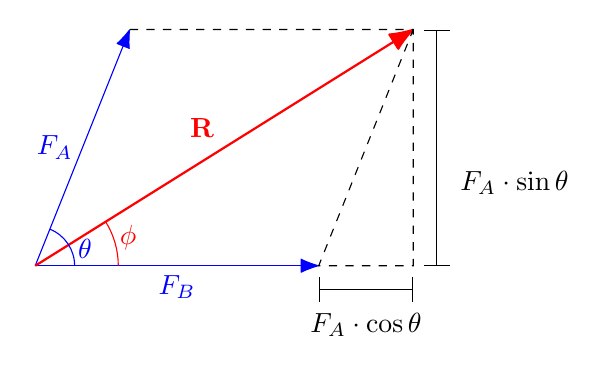
\begin{tikzpicture}[scale=0.6]
            % Forces
            \draw [<-,blue] (2,5) coordinate (C) -- (0,0) node[midway,left] {$F_A$};
            \draw [->,blue] (0,0) coordinate (B) -- (6,0) coordinate (A) node[midway, below] {$F_B$};
            \draw [->,red,thick] (0,0) -- (8,5) coordinate (D) node[midway,above left] {$\mathbf{R}$};

            \draw pic [draw,blue] {angle=A--B--C} node[blue,above=6pt,right=12pt] {$\theta$};
            \draw pic [draw,red,angle radius=30pt] {angle=A--B--D} node[red,above=10pt,right=27pt] {$\phi$};

            \draw [dashed] (2,5) -- (8,5) -- (6,0) -- (8,0) -- (8,5);
            \draw [{Bar[scale=2]}-{Bar[scale=2]}] (6,-0.5) -- (8,-0.5) node[midway,below=5pt] {$F_A\cdot\cos\theta$};
            \draw [{Bar[scale=2]}-{Bar[scale=2]}] (8.5,0) -- (8.5,5) node[midway,below right=5pt] {$F_A\cdot\sin\theta$};
        \end{tikzpicture}
    \end{wrapfigure}

    \begin{flalign*}
        R_x &= F_B + F_A\cdot\cos\theta &&\\
        R_y &= F_A\cdot\sin\theta
    \end{flalign*}
    By the Pythagorean Theorem,
    \begin{flalign*}
        R^2 &= {R_x}^2 + {R_y}^2 &&\\
        &= (F_B + F_A\cdot\cos\theta)^2 + {F_A}^2\cdot\sin^2\theta &&\\
        &= ({F_B}^2 + {F_A}^2\cdot\cos^2\theta + 2 F_B F_A\cdot\cos\theta) + {F_A}^2\cdot\sin^2\theta &&\\
        &= {F_B}^2 + {F_A}^2\cdot(\cos^2\theta + \sin^2\theta)+ 2 F_B F_A\cdot\cos\theta &&\\
        &= {F_A}^2 + {F_B}^2 + 2 F_A F_B\cdot\cos\theta
    \end{flalign*}
    $\therefore$~, the magnitude and direction of the resultant of the two forces is:\\

    % I don't know why the center environment isn't working
    % (it centers at half the width, as if the wrapfig hasn't ended)
    \parbox{\textwidth}{\centering
        $\boxed{\bm{R = \sqrt{{F_A}^2 + {F_B}^2 + 2 F_A F_B\cdot\cos\theta}}}$
        \\[10pt]
        $\tan\phi = \frac{R_y}{R_x}$
        \\[10pt]
        $\boxed{\bm{\phi = \tan^{-1}\left(\frac{R_y}{R_x}\right)}}$
    }\\[20pt]

    %------------------------------------------------------------------------------------------------------------------%
    %------------------------------------------------------------------------------------------------------------------%

    \question{Find the magnitude of the two forces, such that if they act at right angles, their resultant is
        $\sqrt{10}$~N. But if they act at $60\degree$, their resultant is $\sqrt{13}$~N.}

    \begin{wrapfigure}[1]{l}{0.5\textwidth}
        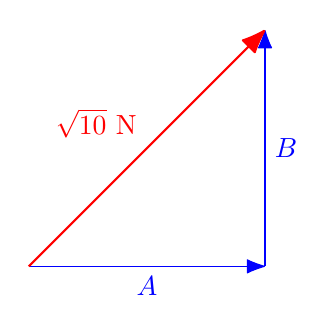
\begin{tikzpicture}[scale=0.6]
            \draw [->,blue] (0,0) -- (5,0) node[midway,below] {$A$};
            \draw [->,blue] (5,0) -- (5,5) node[midway,right] {$B$};
            \draw [->,thick,red] (0,0) -- (5,5) node[midway,above left] {$\sqrt{10}$~N};
        \end{tikzpicture}
        \\[20pt]
        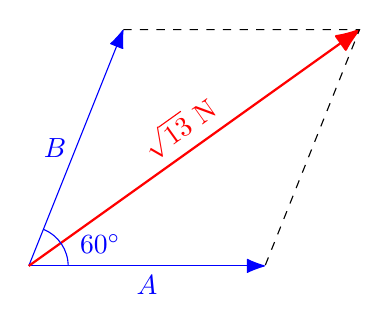
\begin{tikzpicture}[scale=0.6]
            \draw [->,blue] (0,0) -- (5,0) coordinate (A) node[midway,below] {$A$};
            \draw [->,blue] (0,0) coordinate (B) -- (2,5) coordinate (C) node[midway,left] {$B$};
            \draw [->,thick,red] (0,0) -- (7,5) coordinate (D) node[midway,above,sloped] {$\sqrt{13}$~N};

            \draw pic [draw,blue] {angle=A--B--C} node[blue,above=8pt,right=15pt] {$60\degree$};
            \draw [dashed] (2,5) -- (7,5) -- (5,0);
        \end{tikzpicture}
    \end{wrapfigure}\vspace*{-20pt}

    \begin{align}
        A^2 + B^2 &= \left(\sqrt{10}\right)^2 = 10\\
        A^2 + B^2 + 2AB\cdot\cos{60\degree} &= \left(\sqrt{13}\right)^2 = 13\nonumber\\
        A^2 + B^2 + AB &= 13
    \end{align}
    \hspace*{0.3\textwidth}From (1) \& (2),\vspace*{-5pt}
    \begin{align*}
        AB &= 3\\
        (A+B)^2 = A^2 + B^2 + 2AB &= (10) + (2\times{3}) = 16\\
        A+B &= 4
    \end{align*}
    \hspace*{0.3\textwidth}Similarly,\vspace*{-5pt}
    \begin{align*}
        A-B &= 2
    \end{align*}\vspace*{-20pt}
    \parbox{\textwidth}{\centering
        $\bm{\boxed{A = 3~\text{N}}\boxed{B = 1~\text{N}}}$
    }
    \cleardoublepage

    %------------------------------------------------------------------------------------------------------------------%
    %------------------------------------------------------------------------------------------------------------------%

    \question{State following principles:\\\vspace*{-20pt}
        \begin{enumerate}[(a)]
            \item Principle of transmissibility of forces
            \item Principle of superposition of forces
        \end{enumerate}}

    \noindent \underline{Principle of transmissibility of forces} states that if a force acts at any point on a rigid
    body, it may also be considered to act at any other point on its line of action, provided this point is rigidly
    connected with the body.\\

    \noindent\underline{Principle of superposition of forces} states that the combined effect of a force system acting
    on a particle or a rigid body is the sum of the effects of the individual forces.\\

    %------------------------------------------------------------------------------------------------------------------%
    %------------------------------------------------------------------------------------------------------------------%

    \question{A system of four forces acting at a point on a body is as shown in the figure:}\vspace*{-20pt}
    \begin{center}
        \begin{tikzpicture}
            \draw [dashed,Stealth-Stealth] (-3,0) coordinate (X) -- (5,0) node[right] {$x$};
            \draw [dashed,Stealth-Stealth] (0,-3) coordinate (Y) -- (0,4) node[above] {$y$};

            \draw [->] (0,0) -- (4,2) node[above] {$200$~N};
            \draw [->,scale=0.6] (0,0) -- (-3,4) node[above] {$120$~N};
            \draw [->] (0,0) coordinate (B) -- ++(240:1.5) coordinate (A) node[below] {$50$~N};
            \draw [->] (0,0) -- ++(310:3) coordinate (P) node[below] {$100$~N};

            \draw (1.5,0.75) -- (3,0.75) node[midway,below] {$2$} -- (3,1.5) node[midway,right] {$1$};
            \draw [scale=0.8] (-0.5,0.66) -- (-1.5,0.66) node[midway,below] {$3$} -- (-1.5,2) node[midway,left] {$4$};
            \draw pic [draw] {angle=X--B--A} node[midway,below left=8pt] {$60\degree$};
            \draw pic [draw] {angle=Y--B--P} node[midway,below=30pt,right] {$40\degree$};
        \end{tikzpicture}
    \end{center}
    Let $R$ be the resultant force with $R_x$ being the horizontal component and $R_y$ being the vertical component,
    \begin{align*}
        R_x &= 200\cdot\cos{26.56\degree} + 100\cdot\sin{40\degree} -
        (120\cdot\cos{53.13\degree} + 50\cdot\cos{60\degree})\\
        &= \bm{146.17}~\textbf{N}\\
        R_y &= 200\cdot\sin{26.56\degree} + 120\cdot\sin{53.13\degree} -
        (50\cdot\sin{60\degree} + 100\cdot\cos{40\degree})\\
        &= \bm{65.52}~\textbf{N}\\
        R &= \sqrt{(R_x)^2 + (R_y)^2} = \sqrt{21365.66 + 4293.01}\\
        \Aboxed{\bm{R} &= \bm{160.18}~\textbf{N}}\\
        \theta{_R} &= \tan^{-1}\left(\frac{R_y}{R_x}\right) = \tan^{-1}\left(\frac{65.52}{146.17}\right)\\
        \Aboxed{\bm{\theta{_R}} &= \bm{24.14\degree}}
    \end{align*}
    \newpage

    %------------------------------------------------------------------------------------------------------------------%
    %------------------------------------------------------------------------------------------------------------------%

    \question{What is force. State its effect and characteristics.}
    Force can be defined as a push or a pull on an object, it can alter the state of motion of an object.
    \begin{center}
        $F = m\cdot{a}$
    \end{center}

    \noindent{Characteristics \& effects:}
    \begin{enumerate}
        \item It can change the state of motion in an object, i.e., bring an object at rest in motion or vice-versa.
        \item Force always has a magnitude and direction.
        \item The resultant of multiple forces can be calculated by adding the individual forces with vector algebra.
    \end{enumerate}
\end{document}